\documentclass[]{article}
\usepackage{lmodern}
\usepackage{amssymb,amsmath}
\usepackage{ifxetex,ifluatex}
\usepackage{fixltx2e} % provides \textsubscript
\ifnum 0\ifxetex 1\fi\ifluatex 1\fi=0 % if pdftex
  \usepackage[T1]{fontenc}
  \usepackage[utf8]{inputenc}
\else % if luatex or xelatex
  \ifxetex
    \usepackage{mathspec}
  \else
    \usepackage{fontspec}
  \fi
  \defaultfontfeatures{Ligatures=TeX,Scale=MatchLowercase}
\fi
% use upquote if available, for straight quotes in verbatim environments
\IfFileExists{upquote.sty}{\usepackage{upquote}}{}
% use microtype if available
\IfFileExists{microtype.sty}{%
\usepackage{microtype}
\UseMicrotypeSet[protrusion]{basicmath} % disable protrusion for tt fonts
}{}
\usepackage[margin=1in]{geometry}
\usepackage{hyperref}
\hypersetup{unicode=true,
            pdftitle={Titanic Survival Part 1: EDA in R},
            pdfauthor={Marcelo Sanches},
            pdfborder={0 0 0},
            breaklinks=true}
\urlstyle{same}  % don't use monospace font for urls
\usepackage{color}
\usepackage{fancyvrb}
\newcommand{\VerbBar}{|}
\newcommand{\VERB}{\Verb[commandchars=\\\{\}]}
\DefineVerbatimEnvironment{Highlighting}{Verbatim}{commandchars=\\\{\}}
% Add ',fontsize=\small' for more characters per line
\usepackage{framed}
\definecolor{shadecolor}{RGB}{248,248,248}
\newenvironment{Shaded}{\begin{snugshade}}{\end{snugshade}}
\newcommand{\KeywordTok}[1]{\textcolor[rgb]{0.13,0.29,0.53}{\textbf{#1}}}
\newcommand{\DataTypeTok}[1]{\textcolor[rgb]{0.13,0.29,0.53}{#1}}
\newcommand{\DecValTok}[1]{\textcolor[rgb]{0.00,0.00,0.81}{#1}}
\newcommand{\BaseNTok}[1]{\textcolor[rgb]{0.00,0.00,0.81}{#1}}
\newcommand{\FloatTok}[1]{\textcolor[rgb]{0.00,0.00,0.81}{#1}}
\newcommand{\ConstantTok}[1]{\textcolor[rgb]{0.00,0.00,0.00}{#1}}
\newcommand{\CharTok}[1]{\textcolor[rgb]{0.31,0.60,0.02}{#1}}
\newcommand{\SpecialCharTok}[1]{\textcolor[rgb]{0.00,0.00,0.00}{#1}}
\newcommand{\StringTok}[1]{\textcolor[rgb]{0.31,0.60,0.02}{#1}}
\newcommand{\VerbatimStringTok}[1]{\textcolor[rgb]{0.31,0.60,0.02}{#1}}
\newcommand{\SpecialStringTok}[1]{\textcolor[rgb]{0.31,0.60,0.02}{#1}}
\newcommand{\ImportTok}[1]{#1}
\newcommand{\CommentTok}[1]{\textcolor[rgb]{0.56,0.35,0.01}{\textit{#1}}}
\newcommand{\DocumentationTok}[1]{\textcolor[rgb]{0.56,0.35,0.01}{\textbf{\textit{#1}}}}
\newcommand{\AnnotationTok}[1]{\textcolor[rgb]{0.56,0.35,0.01}{\textbf{\textit{#1}}}}
\newcommand{\CommentVarTok}[1]{\textcolor[rgb]{0.56,0.35,0.01}{\textbf{\textit{#1}}}}
\newcommand{\OtherTok}[1]{\textcolor[rgb]{0.56,0.35,0.01}{#1}}
\newcommand{\FunctionTok}[1]{\textcolor[rgb]{0.00,0.00,0.00}{#1}}
\newcommand{\VariableTok}[1]{\textcolor[rgb]{0.00,0.00,0.00}{#1}}
\newcommand{\ControlFlowTok}[1]{\textcolor[rgb]{0.13,0.29,0.53}{\textbf{#1}}}
\newcommand{\OperatorTok}[1]{\textcolor[rgb]{0.81,0.36,0.00}{\textbf{#1}}}
\newcommand{\BuiltInTok}[1]{#1}
\newcommand{\ExtensionTok}[1]{#1}
\newcommand{\PreprocessorTok}[1]{\textcolor[rgb]{0.56,0.35,0.01}{\textit{#1}}}
\newcommand{\AttributeTok}[1]{\textcolor[rgb]{0.77,0.63,0.00}{#1}}
\newcommand{\RegionMarkerTok}[1]{#1}
\newcommand{\InformationTok}[1]{\textcolor[rgb]{0.56,0.35,0.01}{\textbf{\textit{#1}}}}
\newcommand{\WarningTok}[1]{\textcolor[rgb]{0.56,0.35,0.01}{\textbf{\textit{#1}}}}
\newcommand{\AlertTok}[1]{\textcolor[rgb]{0.94,0.16,0.16}{#1}}
\newcommand{\ErrorTok}[1]{\textcolor[rgb]{0.64,0.00,0.00}{\textbf{#1}}}
\newcommand{\NormalTok}[1]{#1}
\usepackage{graphicx,grffile}
\makeatletter
\def\maxwidth{\ifdim\Gin@nat@width>\linewidth\linewidth\else\Gin@nat@width\fi}
\def\maxheight{\ifdim\Gin@nat@height>\textheight\textheight\else\Gin@nat@height\fi}
\makeatother
% Scale images if necessary, so that they will not overflow the page
% margins by default, and it is still possible to overwrite the defaults
% using explicit options in \includegraphics[width, height, ...]{}
\setkeys{Gin}{width=\maxwidth,height=\maxheight,keepaspectratio}
\IfFileExists{parskip.sty}{%
\usepackage{parskip}
}{% else
\setlength{\parindent}{0pt}
\setlength{\parskip}{6pt plus 2pt minus 1pt}
}
\setlength{\emergencystretch}{3em}  % prevent overfull lines
\providecommand{\tightlist}{%
  \setlength{\itemsep}{0pt}\setlength{\parskip}{0pt}}
\setcounter{secnumdepth}{0}
% Redefines (sub)paragraphs to behave more like sections
\ifx\paragraph\undefined\else
\let\oldparagraph\paragraph
\renewcommand{\paragraph}[1]{\oldparagraph{#1}\mbox{}}
\fi
\ifx\subparagraph\undefined\else
\let\oldsubparagraph\subparagraph
\renewcommand{\subparagraph}[1]{\oldsubparagraph{#1}\mbox{}}
\fi

%%% Use protect on footnotes to avoid problems with footnotes in titles
\let\rmarkdownfootnote\footnote%
\def\footnote{\protect\rmarkdownfootnote}

%%% Change title format to be more compact
\usepackage{titling}

% Create subtitle command for use in maketitle
\newcommand{\subtitle}[1]{
  \posttitle{
    \begin{center}\large#1\end{center}
    }
}

\setlength{\droptitle}{-2em}

  \title{Titanic Survival Part 1: EDA in R}
    \pretitle{\vspace{\droptitle}\centering\huge}
  \posttitle{\par}
    \author{Marcelo Sanches}
    \preauthor{\centering\large\emph}
  \postauthor{\par}
      \predate{\centering\large\emph}
  \postdate{\par}
    \date{July 4, 2019}


\begin{document}
\maketitle

\section{Contents}\label{contents}

\begin{itemize}
\tightlist
\item
  Summary
\item
  Preliminary EDA
\item
  Pre-Processing 1: PassengerId, Survived, Pclass
\item
  Pre-Processing 2: Name, Sex
\item
  Pre-Processing 3: SibSp, Parch
\item
  Pre-Processing 4: Ticket, Fare
\item
  Pre-Processing 5: Cabin, Embarked
\item
  Pre-Processing 6: Age
\item
  Univariate Graphical EDA
\item
  Bivariate Graphical EDA
\item
  Multivariate Graphical EDA
\item
  Conclusion
\end{itemize}

\begin{center}\rule{0.5\linewidth}{\linethickness}\end{center}

\section{Summary}\label{summary}

\subsection{Motivation}\label{motivation}

The \textbf{Titanic Survival Project} was born out of my desire not only
to participate in a Kaggle competition but also do avoid the common
mistake of overfitting the test set by submitting various predictions.
In a realistic production environment, the test set would be future data
that we would run a single prediction on, not a playground for getting
better at prediction outcomes of that particular set of data.

I also wanted to use \textbf{R} and \textbf{Python} and play to their
strengths: R for \textbf{data exploration} and \textbf{quick
visualizations}, and Python for \textbf{machine-learning pipelines} and
\textbf{production code}.

\subsection{Project Parts}\label{project-parts}

In \textbf{Part 1} of the Titanic Survival project I conduct
\textbf{Exploratory Data Analisys (EDA)} of the
\href{https://www.kaggle.com/c/titanic/data}{Kaggle Titanic train
dataset} in R, creating an \textbf{RMarkdown report} with RStudio and
the \texttt{knitr} package, with summary tables and visualizations,
performing minor pre-processing as needed.

In \textbf{Part 2} of the project I perform all the necessary
pre-processing steps for Machine Learning models, conduct model
evaluation and regularization, and run predictions using Python in a
\textbf{Jupyter Notebook}. Given a final model, I run a \textbf{single
pipeline} for \textbf{pre-processing and modeling} that emulates a
production environment, where the Titanic test set is used as if it were
future data never before seen.

\subsection{Part 1 Sections}\label{part-1-sections}

In the \textbf{Contents} we can see how \textbf{Part 1} is divided into
several sections. After a \textbf{preliminary EDA} we spend most of our
time \textbf{pre-processing} the data, as usual, and then spend a fair
amount of time exploring it through \textbf{visualizations}. I tried to
organize this exploration into \textbf{univariate, bivariate,} and
\textbf{multivariate} sub-sections, fully aware that the number of
possible combinations quickly explodes even with a few attributes, so
this exploration is still mostly ad hoc.

\begin{center}\rule{0.5\linewidth}{\linethickness}\end{center}

\section{Preliminary EDA}\label{preliminary-eda}

First we load the training data and look at its structure, summary, top
and bottom rows. We will not look at the test data until it is time to
test; failing to do so would consist in \emph{data snooping}. In the
spirit of the Titanic Kaggle kernel, I added the Kaggle Titanic datasets
a level up on an \texttt{input/} directory.

\begin{verbatim}
## 'data.frame':    891 obs. of  12 variables:
##  $ PassengerId: int  1 2 3 4 5 6 7 8 9 10 ...
##  $ Survived   : int  0 1 1 1 0 0 0 0 1 1 ...
##  $ Pclass     : int  3 1 3 1 3 3 1 3 3 2 ...
##  $ Name       : Factor w/ 891 levels "Abbing, Mr. Anthony",..: 109 191 358 277 16 559 520 629 417 581 ...
##  $ Sex        : Factor w/ 2 levels "female","male": 2 1 1 1 2 2 2 2 1 1 ...
##  $ Age        : num  22 38 26 35 35 NA 54 2 27 14 ...
##  $ SibSp      : int  1 1 0 1 0 0 0 3 0 1 ...
##  $ Parch      : int  0 0 0 0 0 0 0 1 2 0 ...
##  $ Ticket     : Factor w/ 681 levels "110152","110413",..: 524 597 670 50 473 276 86 396 345 133 ...
##  $ Fare       : num  7.25 71.28 7.92 53.1 8.05 ...
##  $ Cabin      : Factor w/ 147 levels "A10","A14","A16",..: NA 82 NA 56 NA NA 130 NA NA NA ...
##  $ Embarked   : Factor w/ 3 levels "C","Q","S": 3 1 3 3 3 2 3 3 3 1 ...
\end{verbatim}

There are 891 passengers and 11 attributes (PassengerId is just an index
not an attribute of a passenger). The attributes are:

\begin{itemize}
\tightlist
\item
  \textbf{Survived}, integer, binary indicator (Survived = 1) and the
  target outcome or dependent variable we are to predict.
\item
  \textbf{Pclass}, integer, an ordinal variable for the passenger class.
\item
  \textbf{Name}, Factor w/ 891 levels (one level per passenger).
\item
  \textbf{Sex}, Factor with two levels: ``female'', ``male''.
\item
  \textbf{Age}, numerical, has 177 missing values coded as \texttt{NA}.
\item
  \textbf{SibSp}, integer, an ordinal variable for the number of
  siblings or spouses.
\item
  \textbf{Parch}, integer, an ordinal variable for the number of parents
  or children.
\item
  \textbf{Ticket}, Factor w/ 681 levels.
\item
  \textbf{Fare}, numerical, is in Pounds Sterling, a proxy for wealth or
  social status.
\item
  \textbf{Cabin}, Factor w/ 147 levels, has 687 missing values.
\item
  \textbf{Embarked}, Factor w/ 3 levels: ``C'', ``Q'', and ``S'' for the
  port of embarkation (Cherbourg, Queenstown, and Southhampton), has 2
  missing values.
\end{itemize}

\begin{center}\rule{0.5\linewidth}{\linethickness}\end{center}

\begin{Shaded}
\begin{Highlighting}[]
\CommentTok{# Preliminary summary}
\KeywordTok{summary}\NormalTok{(train)}
\end{Highlighting}
\end{Shaded}

\begin{verbatim}
##   PassengerId       Survived          Pclass     
##  Min.   :  1.0   Min.   :0.0000   Min.   :1.000  
##  1st Qu.:223.5   1st Qu.:0.0000   1st Qu.:2.000  
##  Median :446.0   Median :0.0000   Median :3.000  
##  Mean   :446.0   Mean   :0.3838   Mean   :2.309  
##  3rd Qu.:668.5   3rd Qu.:1.0000   3rd Qu.:3.000  
##  Max.   :891.0   Max.   :1.0000   Max.   :3.000  
##                                                  
##                                     Name         Sex           Age       
##  Abbing, Mr. Anthony                  :  1   female:314   Min.   : 0.42  
##  Abbott, Mr. Rossmore Edward          :  1   male  :577   1st Qu.:20.12  
##  Abbott, Mrs. Stanton (Rosa Hunt)     :  1                Median :28.00  
##  Abelson, Mr. Samuel                  :  1                Mean   :29.70  
##  Abelson, Mrs. Samuel (Hannah Wizosky):  1                3rd Qu.:38.00  
##  Adahl, Mr. Mauritz Nils Martin       :  1                Max.   :80.00  
##  (Other)                              :885                NA's   :177    
##      SibSp           Parch             Ticket         Fare       
##  Min.   :0.000   Min.   :0.0000   1601    :  7   Min.   :  0.00  
##  1st Qu.:0.000   1st Qu.:0.0000   347082  :  7   1st Qu.:  7.91  
##  Median :0.000   Median :0.0000   CA. 2343:  7   Median : 14.45  
##  Mean   :0.523   Mean   :0.3816   3101295 :  6   Mean   : 32.20  
##  3rd Qu.:1.000   3rd Qu.:0.0000   347088  :  6   3rd Qu.: 31.00  
##  Max.   :8.000   Max.   :6.0000   CA 2144 :  6   Max.   :512.33  
##                                   (Other) :852                   
##          Cabin     Embarked  
##  B96 B98    :  4   C   :168  
##  C23 C25 C27:  4   Q   : 77  
##  G6         :  4   S   :644  
##  C22 C26    :  3   NA's:  2  
##  D          :  3             
##  (Other)    :186             
##  NA's       :687
\end{verbatim}

This first summary of our data is not very useful and helps us determine
how to proceed with data pre-processing, converting appropriate
variables into categorical format, cleaning up variables and imputing
missing values as needed. I will refrain from commenting on the data
until pre-processing is mostly finished.

The large number of missing values in \texttt{Cabin} and \texttt{Age}
will need to be dealt with. The 2 missing values in \texttt{Embarked}
can be filled in with the most common port of embarkation.

A look at the dataset helps us get a feel for it:

\begin{Shaded}
\begin{Highlighting}[]
\KeywordTok{head}\NormalTok{(train)}
\end{Highlighting}
\end{Shaded}

\begin{verbatim}
##   PassengerId Survived Pclass
## 1           1        0      3
## 2           2        1      1
## 3           3        1      3
## 4           4        1      1
## 5           5        0      3
## 6           6        0      3
##                                                  Name    Sex Age SibSp
## 1                             Braund, Mr. Owen Harris   male  22     1
## 2 Cumings, Mrs. John Bradley (Florence Briggs Thayer) female  38     1
## 3                              Heikkinen, Miss. Laina female  26     0
## 4        Futrelle, Mrs. Jacques Heath (Lily May Peel) female  35     1
## 5                            Allen, Mr. William Henry   male  35     0
## 6                                    Moran, Mr. James   male  NA     0
##   Parch           Ticket    Fare Cabin Embarked
## 1     0        A/5 21171  7.2500  <NA>        S
## 2     0         PC 17599 71.2833   C85        C
## 3     0 STON/O2. 3101282  7.9250  <NA>        S
## 4     0           113803 53.1000  C123        S
## 5     0           373450  8.0500  <NA>        S
## 6     0           330877  8.4583  <NA>        Q
\end{verbatim}

\begin{Shaded}
\begin{Highlighting}[]
\KeywordTok{tail}\NormalTok{(train)}
\end{Highlighting}
\end{Shaded}

\begin{verbatim}
##     PassengerId Survived Pclass                                     Name
## 886         886        0      3     Rice, Mrs. William (Margaret Norton)
## 887         887        0      2                    Montvila, Rev. Juozas
## 888         888        1      1             Graham, Miss. Margaret Edith
## 889         889        0      3 Johnston, Miss. Catherine Helen "Carrie"
## 890         890        1      1                    Behr, Mr. Karl Howell
## 891         891        0      3                      Dooley, Mr. Patrick
##        Sex Age SibSp Parch     Ticket   Fare Cabin Embarked
## 886 female  39     0     5     382652 29.125  <NA>        Q
## 887   male  27     0     0     211536 13.000  <NA>        S
## 888 female  19     0     0     112053 30.000   B42        S
## 889 female  NA     1     2 W./C. 6607 23.450  <NA>        S
## 890   male  26     0     0     111369 30.000  C148        C
## 891   male  32     0     0     370376  7.750  <NA>        Q
\end{verbatim}

\begin{center}\rule{0.5\linewidth}{\linethickness}\end{center}

\section{Pre-Processing 1: PassengerId, Survived,
Pclass}\label{pre-processing-1-passengerid-survived-pclass}

\subsection{PassengerId}\label{passengerid}

\texttt{PassengerId} is just an index. Since R keeps a row index and we
shouldn't use this variable for modeling as it provides no information,
we drop it, but first check that is has no duplicates and has stepwise
values to ensure data integrity (see ``trust but verify'' code chunk in
the Appendix).

\subsection{Survived}\label{survived}

\texttt{Survived} is dropped and \texttt{SurvivedFac} (as categorical
outcome) and \texttt{SurvivedNum} (as a continuous range from 0 to 1,
indicating probabilities) are created.

\begin{Shaded}
\begin{Highlighting}[]
\CommentTok{# Survived}
\NormalTok{train}\OperatorTok{$}\NormalTok{SurvivedFac <-}\StringTok{ }\KeywordTok{ifelse}\NormalTok{(train}\OperatorTok{$}\NormalTok{Survived}\OperatorTok{==}\StringTok{"1"}\NormalTok{,}\StringTok{"yes"}\NormalTok{,}\StringTok{"no"}\NormalTok{)}
\NormalTok{train}\OperatorTok{$}\NormalTok{SurvivedFac <-}\StringTok{ }\KeywordTok{factor}\NormalTok{(train}\OperatorTok{$}\NormalTok{Survived, }\DataTypeTok{levels=}\DecValTok{0}\OperatorTok{:}\DecValTok{1}\NormalTok{, }\DataTypeTok{labels=}\KeywordTok{c}\NormalTok{(}\StringTok{"no"}\NormalTok{,}\StringTok{"yes"}\NormalTok{))}
\NormalTok{train}\OperatorTok{$}\NormalTok{SurvivedNum <-}\StringTok{ }\KeywordTok{as.numeric}\NormalTok{(train}\OperatorTok{$}\NormalTok{Survived) }
\NormalTok{train}\OperatorTok{$}\NormalTok{Survived <-}\StringTok{ }\OtherTok{NULL} \CommentTok{# drop original}
\end{Highlighting}
\end{Shaded}

\subsection{Pclass}\label{pclass}

\texttt{Pclass} is dropped and \texttt{PclassFac} (as categorical) and
\texttt{PclassNum} (as ordinal) are created. The former is useful for
plotting, the latter for machine learning.

\begin{Shaded}
\begin{Highlighting}[]
\CommentTok{# Pclass}
\NormalTok{train}\OperatorTok{$}\NormalTok{PclassFac <-}\StringTok{ }\KeywordTok{ifelse}\NormalTok{(train}\OperatorTok{$}\NormalTok{Pclass}\OperatorTok{==}\DecValTok{1}\NormalTok{, }\StringTok{"1st Class"}\NormalTok{, }\KeywordTok{ifelse}\NormalTok{(train}\OperatorTok{$}\NormalTok{Pclass}\OperatorTok{==}\DecValTok{2}\NormalTok{, }\StringTok{"2nd Class"}\NormalTok{, }\StringTok{"3rd Class"}\NormalTok{))}
\NormalTok{train}\OperatorTok{$}\NormalTok{PclassFac <-}\StringTok{ }\KeywordTok{factor}\NormalTok{(train}\OperatorTok{$}\NormalTok{PclassFac)}
\NormalTok{train}\OperatorTok{$}\NormalTok{PclassNum <-}\StringTok{ }\KeywordTok{as.integer}\NormalTok{(train}\OperatorTok{$}\NormalTok{Pclass)}
\NormalTok{train}\OperatorTok{$}\NormalTok{Pclass <-}\StringTok{ }\OtherTok{NULL}
\end{Highlighting}
\end{Shaded}

\begin{center}\rule{0.5\linewidth}{\linethickness}\end{center}

\section{Pre-Processing 2: Name, Sex}\label{pre-processing-2-name-sex}

The \texttt{Name} attribute is not indicative of a person's survival,
yet information can be extracted from it such as titles and name
lengths, which might contain some predictive power.

A \texttt{Title} attribute can be created by extracting titles with
regular expresssions.

\subsection{Title}\label{title}

\begin{Shaded}
\begin{Highlighting}[]
\CommentTok{# Create Title attribute}
\NormalTok{train}\OperatorTok{$}\NormalTok{Title <-}\StringTok{ }\KeywordTok{vector}\NormalTok{(}\StringTok{"character"}\NormalTok{,}\DataTypeTok{length=}\KeywordTok{nrow}\NormalTok{(train))}
\ControlFlowTok{for}\NormalTok{ (i }\ControlFlowTok{in} \DecValTok{1}\OperatorTok{:}\KeywordTok{nrow}\NormalTok{(train)) \{}
\NormalTok{    x <-}\StringTok{ }\KeywordTok{as.character}\NormalTok{(train}\OperatorTok{$}\NormalTok{Name[i])}
\NormalTok{    m <-}\StringTok{ }\KeywordTok{regexec}\NormalTok{(}\StringTok{",(}\CharTok{\textbackslash{}\textbackslash{}}\StringTok{s+}\CharTok{\textbackslash{}\textbackslash{}}\StringTok{w+)+}\CharTok{\textbackslash{}\textbackslash{}}\StringTok{."}\NormalTok{, x) }
\NormalTok{    train}\OperatorTok{$}\NormalTok{Title[i] <-}\StringTok{ }\KeywordTok{unlist}\NormalTok{(}\KeywordTok{strsplit}\NormalTok{(}\KeywordTok{unlist}\NormalTok{(}\KeywordTok{regmatches}\NormalTok{(x,m)),}\StringTok{" "}\NormalTok{))[}\DecValTok{2}\NormalTok{]}
\NormalTok{\}}
\CommentTok{# looking at unique titles}
\KeywordTok{unique}\NormalTok{(train}\OperatorTok{$}\NormalTok{Title)}
\end{Highlighting}
\end{Shaded}

\begin{verbatim}
##  [1] "Mr."       "Mrs."      "Miss."     "Master."   "Don."     
##  [6] "Rev."      "Dr."       "Mme."      "Ms."       "Major."   
## [11] "Lady."     "Sir."      "Mlle."     "Col."      "Capt."    
## [16] "the"       "Jonkheer."
\end{verbatim}

There are 17 levels which seem unnecessary as some of these titles are
specific and rare, so we can bin them into two rare categories, one for
males and one for females, since the probability of survival is highly
dependent on gender.

I will not fix the title \textbf{the}, which stands for \textbf{the
Countess}, since any specific fixes will not be generalizable to any
future data (aka the test set) in production. Instead, I am hoping no
other specific male titles (such as \textbf{the Count}) will pop up in
the test data and will use the above rare male titles as baseline for
the rare cases, all other rare cases will end up in the rare female
bucket.

Note that some decisions are simplifications, there is a female doctor
(Dr.~Alice Leader) yet I assigned `Dr.' to the rare male title category
since at that time most doctors were males.

\begin{Shaded}
\begin{Highlighting}[]
\CommentTok{# Clean up Title}
\NormalTok{common_titles <-}\StringTok{ }\KeywordTok{c}\NormalTok{(}\StringTok{"Mr."}\NormalTok{, }\StringTok{"Mrs."}\NormalTok{, }\StringTok{"Miss."}\NormalTok{)}
\NormalTok{rare_male <-}\StringTok{ }\KeywordTok{c}\NormalTok{(}\StringTok{"Don."}\NormalTok{,}\StringTok{"Rev."}\NormalTok{,}\StringTok{"Dr."}\NormalTok{,}\StringTok{"Major."}\NormalTok{,}\StringTok{"Master."}\NormalTok{, }\StringTok{"Sir."}\NormalTok{,}\StringTok{"Col."}\NormalTok{,}\StringTok{"Capt."}\NormalTok{,}\StringTok{"Jonkheer."}\NormalTok{)}
\ControlFlowTok{for}\NormalTok{ (i }\ControlFlowTok{in} \DecValTok{1}\OperatorTok{:}\KeywordTok{nrow}\NormalTok{(train)) \{}
\NormalTok{    train}\OperatorTok{$}\NormalTok{Title[i] <-}\StringTok{ }\KeywordTok{ifelse}\NormalTok{(train}\OperatorTok{$}\NormalTok{Title[i] }\OperatorTok\StringTok{ }\NormalTok{common_titles, train}\OperatorTok{$}\NormalTok{Title[i], }\CommentTok{# do not replace}
                             \KeywordTok{ifelse}\NormalTok{(train}\OperatorTok{$}\NormalTok{Title[i] }\OperatorTok\StringTok{ }\NormalTok{rare_male, }\StringTok{"rareMale"}\NormalTok{, }\StringTok{"rareFemale"}\NormalTok{))}
\NormalTok{\}}
\NormalTok{train}\OperatorTok{$}\NormalTok{Title <-}\StringTok{ }\KeywordTok{factor}\NormalTok{(train}\OperatorTok{$}\NormalTok{Title)}
\CommentTok{# unique titles}
\KeywordTok{unique}\NormalTok{(train}\OperatorTok{$}\NormalTok{Title)}
\end{Highlighting}
\end{Shaded}

\begin{verbatim}
## [1] Mr.        Mrs.       Miss.      rareMale   rareFemale
## Levels: Miss. Mr. Mrs. rareFemale rareMale
\end{verbatim}

Before dropping name entirely, we can informally test a common
assumption that the length of a name is associated positively with
higher socio-economic status and therefore survivability. (See Appendix
for the \texttt{NameLength} code.)

\subsection{NameLength}\label{namelength}

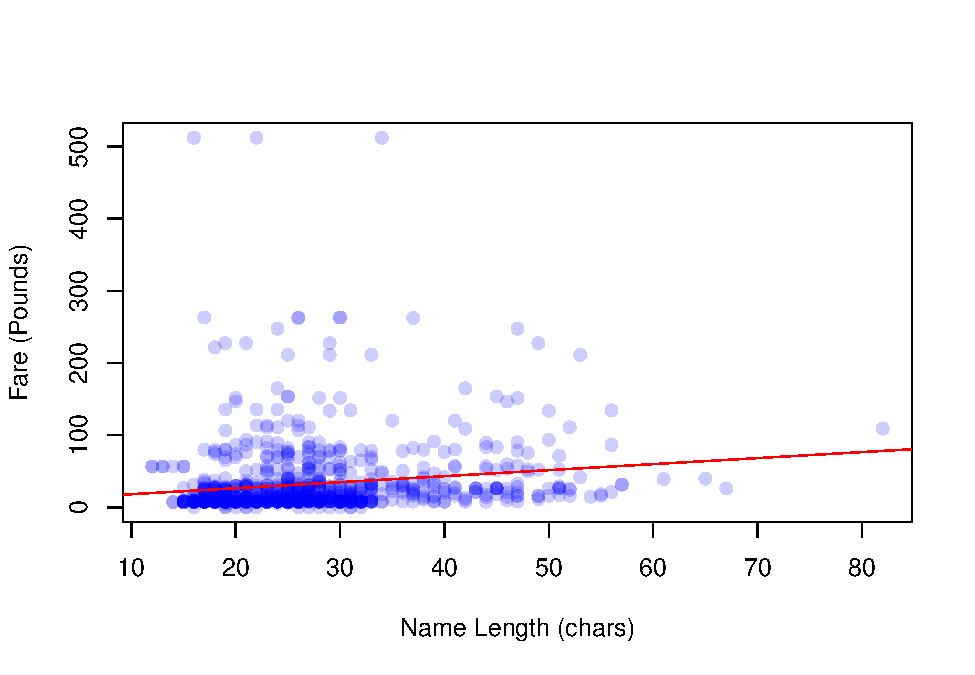
\includegraphics{Titanic_Survival_files/figure-latex/unnamed-chunk-10-1.pdf}

While the evidence isn't particularly strong, we might as well keep
\texttt{NameLength} in the mix just to see whether it improves modeling
later on. Now we could drop \texttt{Name}, but will do so after some
further cleaning as we use this for EDA later.

\subsection{Sex: GenederFac, IsMale}\label{sex-genederfac-ismale}

The variable \texttt{Sex} is usually best represented as a binary
indicator for a given gender in machine learning, however, for plotting
purposes we keep a categorical representation, creating
\texttt{GenderFac} and \texttt{IsMale} wherein Male=1.

\begin{Shaded}
\begin{Highlighting}[]
\NormalTok{train}\OperatorTok{$}\NormalTok{GenderFac <-}\StringTok{ }\NormalTok{train}\OperatorTok{$}\NormalTok{Sex }\CommentTok{# factor for plotting}
\NormalTok{train}\OperatorTok{$}\NormalTok{IsMale <-}\StringTok{ }\KeywordTok{ifelse}\NormalTok{(train}\OperatorTok{$}\NormalTok{Sex}\OperatorTok{==}\StringTok{"male"}\NormalTok{,}\DecValTok{1}\NormalTok{,}\DecValTok{0}\NormalTok{) }\CommentTok{# indicator for ML}
\NormalTok{train}\OperatorTok{$}\NormalTok{Sex <-}\StringTok{ }\OtherTok{NULL} \CommentTok{# drop original}
\end{Highlighting}
\end{Shaded}

\begin{center}\rule{0.5\linewidth}{\linethickness}\end{center}

\section{Pre-Processing 3: SibSp,
Parch}\label{pre-processing-3-sibsp-parch}

We conveniently rename \texttt{SibSp} and \texttt{Parch} to
\texttt{SiblingSpouse} and \texttt{ParentChildren} and create a variable
that is a sum of the two: \texttt{NumRelatives}.

\begin{Shaded}
\begin{Highlighting}[]
\CommentTok{# Change SibSp and Parch to factor}
\NormalTok{train}\OperatorTok{$}\NormalTok{SiblingSpouse <-}\StringTok{ }\KeywordTok{factor}\NormalTok{(train}\OperatorTok{$}\NormalTok{SibSp)}
\NormalTok{train}\OperatorTok{$}\NormalTok{ParentChildren <-}\StringTok{ }\KeywordTok{factor}\NormalTok{(train}\OperatorTok{$}\NormalTok{Parch)}
\NormalTok{train}\OperatorTok{$}\NormalTok{NumRelatives <-}\StringTok{ }\NormalTok{train}\OperatorTok{$}\NormalTok{SibSp }\OperatorTok{+}\StringTok{ }\NormalTok{train}\OperatorTok{$}\NormalTok{Parch}
\NormalTok{train}\OperatorTok{$}\NormalTok{NumRelatives <-}\StringTok{ }\KeywordTok{factor}\NormalTok{(train}\OperatorTok{$}\NormalTok{NumRelatives)}
\NormalTok{train}\OperatorTok{$}\NormalTok{SibSp <-}\StringTok{ }\OtherTok{NULL}
\NormalTok{train}\OperatorTok{$}\NormalTok{Parch <-}\StringTok{ }\OtherTok{NULL}
\end{Highlighting}
\end{Shaded}

\begin{center}\rule{0.5\linewidth}{\linethickness}\end{center}

\section{Pre-Processing 4: Ticket,
Fare}\label{pre-processing-4-ticket-fare}

\subsection{Ticket}\label{ticket}

The \texttt{Ticket} attribute is somewhat useless as far as extracting
information from the ticket number itself. What the ticket number does
provide, however, is information on how many tickets were purchased
under a given \texttt{Fare}, such that we can calculate the \textbf{fare
per person}, which is what we need since our observational unit (a row)
is a person.

Here is a sample of how there are repeated ticket numbers under the same
fare:

\begin{Shaded}
\begin{Highlighting}[]
\CommentTok{# EDA into Ticket and Fare}
\NormalTok{temp_dfm <-}\StringTok{ }\NormalTok{train[, }\KeywordTok{colnames}\NormalTok{(train) }\OperatorTok\StringTok{ }\KeywordTok{c}\NormalTok{(}\StringTok{"Name"}\NormalTok{,}\StringTok{"Ticket"}\NormalTok{,}\StringTok{"Fare"}\NormalTok{)]}
\NormalTok{temp_dfm <-}\StringTok{ }\NormalTok{temp_dfm[}\KeywordTok{order}\NormalTok{(temp_dfm[}\StringTok{"Ticket"}\NormalTok{]),] }\CommentTok{# order by Ticket}
\NormalTok{temp_dfm[}\DecValTok{1}\OperatorTok{:}\DecValTok{10}\NormalTok{,]}
\end{Highlighting}
\end{Shaded}

\begin{verbatim}
##                                                         Name Ticket  Fare
## 258                                     Cherry, Miss. Gladys 110152 86.50
## 505                                    Maioni, Miss. Roberta 110152 86.50
## 760 Rothes, the Countess. of (Lucy Noel Martha Dyer-Edwards) 110152 86.50
## 263                                        Taussig, Mr. Emil 110413 79.65
## 559                   Taussig, Mrs. Emil (Tillie Mandelbaum) 110413 79.65
## 586                                      Taussig, Miss. Ruth 110413 79.65
## 111                           Porter, Mr. Walter Chamberlain 110465 52.00
## 476                              Clifford, Mr. George Quincy 110465 52.00
## 431                Bjornstrom-Steffansson, Mr. Mauritz Hakan 110564 26.55
## 367         Warren, Mrs. Frank Manley (Anna Sophia Atkinson) 110813 75.25
\end{verbatim}

There are many cases of families with the same last name (such as the
Taussig above) which leads us to believe that these are not individual
prices but group prices under the same ticket. So we keep
\texttt{Ticket} only to clean fare.

\subsection{Fare}\label{fare}

We create a \texttt{FarePerPerson} attribute and compare it to the
\texttt{Fare} attribute:

\begin{Shaded}
\begin{Highlighting}[]
\CommentTok{# keep counts of tickets}
\NormalTok{counts <-}\StringTok{ }\KeywordTok{aggregate}\NormalTok{(train}\OperatorTok{$}\NormalTok{Ticket, }\DataTypeTok{by=}\KeywordTok{list}\NormalTok{(train}\OperatorTok{$}\NormalTok{Ticket), }
                      \DataTypeTok{FUN=}\ControlFlowTok{function}\NormalTok{(ticket) }\KeywordTok{sum}\NormalTok{(}\OperatorTok{!}\KeywordTok{is.na}\NormalTok{(ticket)))}
\CommentTok{# function that takes a data frame's fare and ticket counts and apply}
\NormalTok{divide_fare_count <-}\StringTok{ }\ControlFlowTok{function}\NormalTok{(dfm) \{}
\NormalTok{  fare <-}\StringTok{ }\KeywordTok{as.numeric}\NormalTok{(dfm[}\StringTok{"Fare"}\NormalTok{])}
  \CommentTok{# ticket counts}
\NormalTok{  count_given_ticket <-}\StringTok{ }\NormalTok{counts[}\KeywordTok{which}\NormalTok{(counts[,}\DecValTok{1}\NormalTok{] }\OperatorTok{==}\StringTok{ }\NormalTok{dfm[}\StringTok{"Ticket"}\NormalTok{]), }\DecValTok{2}\NormalTok{]}
\NormalTok{  result <-}\StringTok{ }\KeywordTok{round}\NormalTok{(fare}\OperatorTok{/}\NormalTok{count_given_ticket,}\DecValTok{2}\NormalTok{)}
  \KeywordTok{return}\NormalTok{(result)}
\NormalTok{\}}
\CommentTok{# create FarePerPerson}
\NormalTok{train}\OperatorTok{$}\NormalTok{FarePerPerson <-}\StringTok{ }\KeywordTok{apply}\NormalTok{(}\DataTypeTok{X=}\NormalTok{train, }\DataTypeTok{MARGIN=}\DecValTok{1}\NormalTok{, }\DataTypeTok{FUN=}\NormalTok{divide_fare_count)}

\CommentTok{# looking at the temp dataframe of results again}
\NormalTok{chosen <-}\StringTok{ }\KeywordTok{c}\NormalTok{(}\StringTok{"Name"}\NormalTok{,}\StringTok{"Ticket"}\NormalTok{,}\StringTok{"Fare"}\NormalTok{,}\StringTok{"FarePerPerson"}\NormalTok{)}
\NormalTok{temp_dfm <-}\StringTok{ }\NormalTok{train[, }\KeywordTok{colnames}\NormalTok{(train) }\OperatorTok\StringTok{ }\NormalTok{chosen]}
\NormalTok{temp_dfm <-}\StringTok{ }\NormalTok{temp_dfm[}\KeywordTok{order}\NormalTok{(temp_dfm[}\StringTok{"Ticket"}\NormalTok{]),] }\CommentTok{# order by Ticket}
\NormalTok{temp_dfm[}\DecValTok{1}\OperatorTok{:}\DecValTok{10}\NormalTok{,]}
\end{Highlighting}
\end{Shaded}

\begin{verbatim}
##                                                         Name Ticket  Fare
## 258                                     Cherry, Miss. Gladys 110152 86.50
## 505                                    Maioni, Miss. Roberta 110152 86.50
## 760 Rothes, the Countess. of (Lucy Noel Martha Dyer-Edwards) 110152 86.50
## 263                                        Taussig, Mr. Emil 110413 79.65
## 559                   Taussig, Mrs. Emil (Tillie Mandelbaum) 110413 79.65
## 586                                      Taussig, Miss. Ruth 110413 79.65
## 111                           Porter, Mr. Walter Chamberlain 110465 52.00
## 476                              Clifford, Mr. George Quincy 110465 52.00
## 431                Bjornstrom-Steffansson, Mr. Mauritz Hakan 110564 26.55
## 367         Warren, Mrs. Frank Manley (Anna Sophia Atkinson) 110813 75.25
##     FarePerPerson
## 258         28.83
## 505         28.83
## 760         28.83
## 263         26.55
## 559         26.55
## 586         26.55
## 111         26.00
## 476         26.00
## 431         26.55
## 367         75.25
\end{verbatim}

We can now drop \texttt{Fare}, \texttt{Name}, and \texttt{Ticket}, but
we can keep the ticket counts as its own attribute \texttt{TicketCount}:

\begin{Shaded}
\begin{Highlighting}[]
\CommentTok{# create TicketCount}
\NormalTok{train}\OperatorTok{$}\NormalTok{TicketCount <-}\StringTok{ }\KeywordTok{apply}\NormalTok{(}\DataTypeTok{X=}\NormalTok{train, }\DataTypeTok{MARGIN=}\DecValTok{1}\NormalTok{, }\DataTypeTok{FUN=}\ControlFlowTok{function}\NormalTok{(dfm) counts[}\KeywordTok{which}\NormalTok{(counts[,}\DecValTok{1}\NormalTok{] }\OperatorTok{==}\StringTok{ }\NormalTok{dfm[}\StringTok{"Ticket"}\NormalTok{]), }\DecValTok{2}\NormalTok{])}
\CommentTok{# drop Fare, Name, and Ticket}
\StringTok{'%ni%'}\NormalTok{ <-}\StringTok{ }\KeywordTok{Negate}\NormalTok{(}\StringTok{'%in%'}\NormalTok{)}
\NormalTok{not_chosen <-}\StringTok{ }\KeywordTok{c}\NormalTok{(}\StringTok{"Fare"}\NormalTok{,}\StringTok{"Name"}\NormalTok{,}\StringTok{"Ticket"}\NormalTok{)}
\NormalTok{train <-}\StringTok{ }\NormalTok{train[,}\KeywordTok{colnames}\NormalTok{(train) }\OperatorTok\StringTok{ }\NormalTok{not_chosen]}
\end{Highlighting}
\end{Shaded}

Since \texttt{FarePerPerson} has a skewed distribution (as we shall see
in the Graphical EDA section) we create a \texttt{FarePerPErsonLog}
variable which will help with linear models.

\begin{Shaded}
\begin{Highlighting}[]
\CommentTok{# create FareLog}
\NormalTok{train}\OperatorTok{$}\NormalTok{FarePerPersonLog <-}\StringTok{ }\KeywordTok{log}\NormalTok{(train}\OperatorTok{$}\NormalTok{FarePerPerson}\OperatorTok{+}\DecValTok{1}\NormalTok{)}
\end{Highlighting}
\end{Shaded}

\begin{Shaded}
\begin{Highlighting}[]
\KeywordTok{names}\NormalTok{(train)}
\end{Highlighting}
\end{Shaded}

\begin{verbatim}
##  [1] "Age"              "Cabin"            "Embarked"        
##  [4] "SurvivedFac"      "SurvivedNum"      "PclassFac"       
##  [7] "PclassNum"        "Title"            "NameLength"      
## [10] "GenderFac"        "IsMale"           "SiblingSpouse"   
## [13] "ParentChildren"   "NumRelatives"     "FarePerPerson"   
## [16] "TicketCount"      "FarePerPersonLog"
\end{verbatim}

\begin{center}\rule{0.5\linewidth}{\linethickness}\end{center}

\section{Pre-Processing 5: Cabin,
Embarked}\label{pre-processing-5-cabin-embarked}

\subsection{Cabin}\label{cabin}

\texttt{Cabin} has 687 NAs and 147 levels yet cabin locations might be
important in determining survivability, since the accident happened late
at night when people were mostly in their cabins, and lower-letter
cabins were near the deck while higher-letter cabins were near the keel
where the ship hit the iceberg.

\begin{Shaded}
\begin{Highlighting}[]
\KeywordTok{summary}\NormalTok{(train}\OperatorTok{$}\NormalTok{Cabin)}
\end{Highlighting}
\end{Shaded}

\begin{verbatim}
##    A    B    C    D    E    F NA's 
##   15   47   59   33   32   18  687
\end{verbatim}

We now have good representations in all cabins and not too many levels
but still a lot of missing values, we'll deal with those later as
needed.

\subsection{Embarked}\label{embarked}

We substitute the letters for port names and impute the two missing
cases with the majority class.

\begin{Shaded}
\begin{Highlighting}[]
\NormalTok{train}\OperatorTok{$}\NormalTok{Embarked <-}\StringTok{ }\KeywordTok{ifelse}\NormalTok{(train}\OperatorTok{$}\NormalTok{Embarked}\OperatorTok{==}\StringTok{"C"}\NormalTok{,}\StringTok{"Cherbourg"}\NormalTok{,}
                         \KeywordTok{ifelse}\NormalTok{(train}\OperatorTok{$}\NormalTok{Embarked}\OperatorTok{==}\StringTok{"Q"}\NormalTok{,}\StringTok{"Queensland"}\NormalTok{,}\StringTok{"Southhampton"}\NormalTok{))}
\NormalTok{train}\OperatorTok{$}\NormalTok{Embarked[}\KeywordTok{is.na}\NormalTok{(train}\OperatorTok{$}\NormalTok{Embarked)] <-}\StringTok{ "Southhampton"}
\NormalTok{train}\OperatorTok{$}\NormalTok{Embarked <-}\StringTok{ }\KeywordTok{factor}\NormalTok{(train}\OperatorTok{$}\NormalTok{Embarked) }\CommentTok{# re-factoring}
\end{Highlighting}
\end{Shaded}

\begin{center}\rule{0.5\linewidth}{\linethickness}\end{center}

\section{Pre-Processing 6: Age}\label{pre-processing-6-age}

\subsection{Imputing Missing Values}\label{imputing-missing-values}

The \texttt{Age} variable had to be considered at the end of
pre-processing since we will be doing some pre-modeling (modeling during
data pre-processing) to impute missing values and needed other variables
to be relatively clean before this pre-modeling stage.

It is helpful to visualize the distribution of ages before and after a
certain imputing strategy to see the effect it has on the data. The
common practice of imputing with measures of center such as the mean or
the median (in our case there wouldn't be much of a difference as the
distribution is approximately normal) distorts the distribution. To show
this effectively, the y axes must agree:

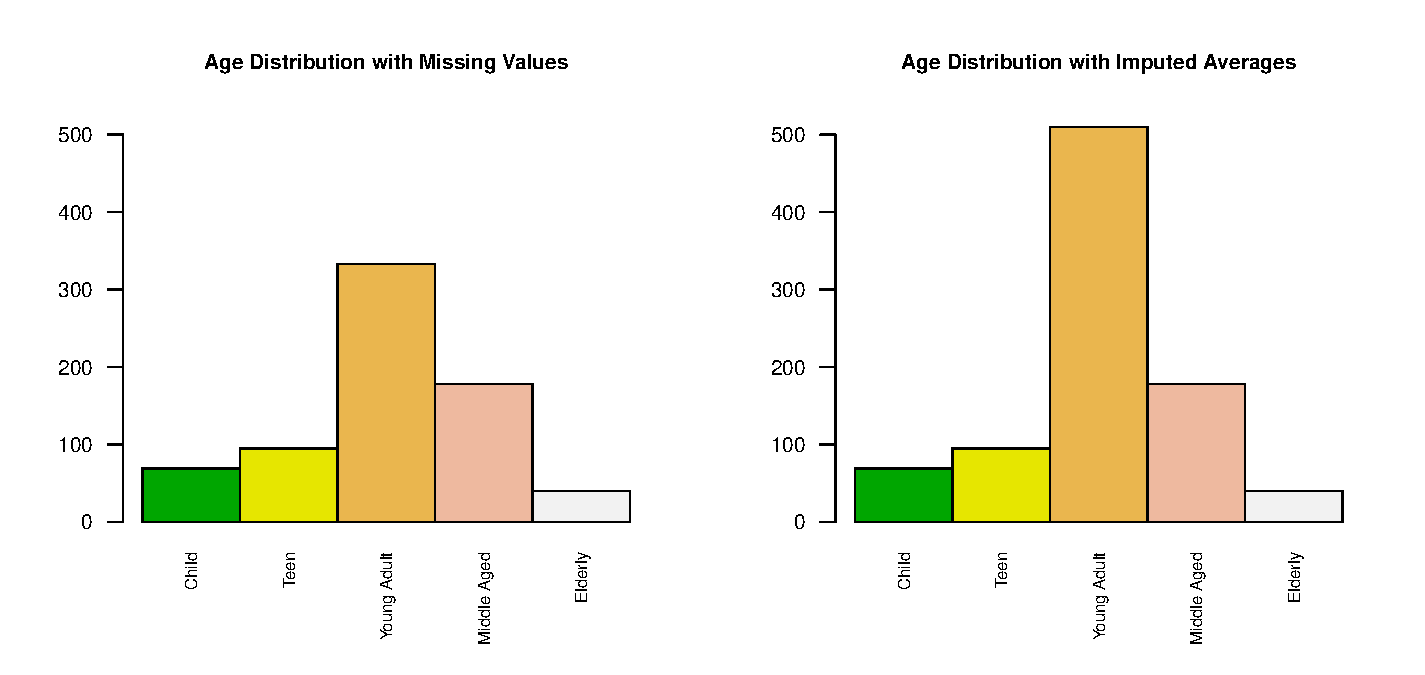
\includegraphics{Titanic_Survival_files/figure-latex/unnamed-chunk-21-1.pdf}

Imputing medians amounts to deciding that when we do not know an age, we
will classify this person as a young adult.

A better strategy would be to \textbf{generate random values} given a
similar distribution to that which we observed in our traning data, yet
one problem with this approach is that it overfits the values we
observe, reinforcing patterns that might not necessarily be
generalizable.

A final and more sophisticated approach would be to use the rest of the
information in the training data and \textbf{predict ages} for those
individuals, based on other attributes. Since Decision Tree models take
missing and unscaled values, and work with categorical features, we can
quickly predict ages with minimal modeling.

First we select features for modeling since we have many redundant
features (such as the logged variables), and separate the data into sets
with age and without age. These features were chosen after a bit of
trial and error and plotting of the variable importance score generated
by the random forest (see below), which allowed me to simplify the model
by removing attributes that weren't helping the model. In short, the
model was too complex and therefore there was too much variance.

\begin{Shaded}
\begin{Highlighting}[]
\CommentTok{# choose features for modeling}
\NormalTok{chosen <-}\StringTok{ }\KeywordTok{c}\NormalTok{(}\StringTok{"Age"}\NormalTok{,}\StringTok{"SurvivedFac"}\NormalTok{,}\StringTok{"PclassFac"}\NormalTok{,}\StringTok{"Title"}\NormalTok{,}\StringTok{"NameLength"}\NormalTok{,}
            \StringTok{"SiblingSpouse"}\NormalTok{,}\StringTok{"ParentChildren"}\NormalTok{,}\StringTok{"FarePerPerson"}\NormalTok{,}\StringTok{"TicketCount"}\NormalTok{)}
\NormalTok{yesAge <-}\StringTok{ }\NormalTok{train[}\OperatorTok{!}\KeywordTok{is.na}\NormalTok{(train}\OperatorTok{$}\NormalTok{Age), }\KeywordTok{colnames}\NormalTok{(train) }\OperatorTok\StringTok{ }\NormalTok{chosen] }\CommentTok{# with ages <- to train and evaluate models}
\NormalTok{noAge <-}\StringTok{ }\NormalTok{train[}\KeywordTok{is.na}\NormalTok{(train}\OperatorTok{$}\NormalTok{Age), }\KeywordTok{colnames}\NormalTok{(train) }\OperatorTok\StringTok{ }\NormalTok{chosen] }\CommentTok{# without ages <- to predict}
\CommentTok{# drop the outcome since it only has missing values}
\NormalTok{noAge}\OperatorTok{$}\NormalTok{Age <-}\StringTok{ }\OtherTok{NULL}
\end{Highlighting}
\end{Shaded}

Now we can use the dataset with ages to train a tree model:

\begin{Shaded}
\begin{Highlighting}[]
\KeywordTok{library}\NormalTok{(tree)}
\KeywordTok{library}\NormalTok{(caTools)}
\KeywordTok{set.seed}\NormalTok{(}\DecValTok{1}\NormalTok{) }
\CommentTok{# split on outcome}
\NormalTok{Y_age <-}\StringTok{ }\NormalTok{yesAge[, }\StringTok{"Age"}\NormalTok{]}
\NormalTok{age_bool <-}\StringTok{ }\KeywordTok{sample.split}\NormalTok{(Y_age, }\DataTypeTok{SplitRatio =} \DecValTok{2}\OperatorTok{/}\DecValTok{3}\NormalTok{) }
\NormalTok{age_train <-}\StringTok{ }\NormalTok{yesAge[age_bool, ]}
\NormalTok{age_test <-}\StringTok{ }\NormalTok{yesAge[}\OperatorTok{!}\NormalTok{age_bool, }\KeywordTok{colnames}\NormalTok{(yesAge) }\OperatorTok{!=}\StringTok{ "Age"}\NormalTok{]}
\CommentTok{# fit model}
\NormalTok{age_mod <-}\StringTok{ }\KeywordTok{tree}\NormalTok{(Age}\OperatorTok{~}\NormalTok{.,}\DataTypeTok{data=}\NormalTok{age_train)}
\CommentTok{# plot tree}
\KeywordTok{plot}\NormalTok{(age_mod)}
\KeywordTok{text}\NormalTok{(age_mod, }\DataTypeTok{pretty=}\DecValTok{0}\NormalTok{)}
\end{Highlighting}
\end{Shaded}

\includegraphics{Titanic_Survival_files/figure-latex/unnamed-chunk-23-1.pdf}

One problem with this single tree approach is that another random
starting point would generate an entirely different tree. Let's how this
single tree did as far as predicting ages in the test set:

\begin{Shaded}
\begin{Highlighting}[]
\NormalTok{y_hat <-}\StringTok{ }\KeywordTok{predict}\NormalTok{(age_mod, }\DataTypeTok{newdata=}\NormalTok{age_test)}
\NormalTok{y_test <-}\StringTok{ }\NormalTok{yesAge[}\OperatorTok{!}\NormalTok{age_bool, }\StringTok{"Age"}\NormalTok{]}
\NormalTok{test_RMSE <-}\StringTok{ }\KeywordTok{round}\NormalTok{(}\KeywordTok{sqrt}\NormalTok{(}\KeywordTok{mean}\NormalTok{((y_hat }\OperatorTok{-}\StringTok{ }\NormalTok{y_test)}\OperatorTok{^}\DecValTok{2}\NormalTok{)),}\DecValTok{2}\NormalTok{)}
\KeywordTok{plot}\NormalTok{(y_hat, y_test,}\DataTypeTok{ylab=}\StringTok{"Actual Age"}\NormalTok{,}\DataTypeTok{xlab=}\StringTok{"Predicted Age"}\NormalTok{,}\DataTypeTok{pch=}\DecValTok{19}\NormalTok{,}\DataTypeTok{col=}\KeywordTok{rgb}\NormalTok{(}\DecValTok{0}\NormalTok{,}\DecValTok{0}\NormalTok{,}\DecValTok{1}\NormalTok{,}\FloatTok{0.3}\NormalTok{))}
\KeywordTok{text}\NormalTok{(}\KeywordTok{c}\NormalTok{(}\DecValTok{35}\NormalTok{,}\DecValTok{40}\NormalTok{),}\DecValTok{10}\NormalTok{, }\KeywordTok{c}\NormalTok{(}\StringTok{"RMSE = "}\NormalTok{, test_RMSE))}
\KeywordTok{abline}\NormalTok{(}\DecValTok{0}\NormalTok{,}\DecValTok{1}\NormalTok{, }\DataTypeTok{col=}\StringTok{"red"}\NormalTok{,}\DataTypeTok{lty=}\DecValTok{2}\NormalTok{)}
\end{Highlighting}
\end{Shaded}

\includegraphics{Titanic_Survival_files/figure-latex/unnamed-chunk-24-1.pdf}

The tree seems to be overpredicting specific ages like 30 and 40 and
making lots of errors because of this. Let's see if an ensemble model
like random forest performs better.

\begin{Shaded}
\begin{Highlighting}[]
\KeywordTok{suppressMessages}\NormalTok{(}\KeywordTok{library}\NormalTok{(randomForest))}
\CommentTok{# split on outcome}
\KeywordTok{set.seed}\NormalTok{(}\DecValTok{1}\NormalTok{)}
\NormalTok{Y_age <-}\StringTok{ }\NormalTok{yesAge[, }\StringTok{"Age"}\NormalTok{]}
\NormalTok{age_bool <-}\StringTok{ }\KeywordTok{sample.split}\NormalTok{(Y_age, }\DataTypeTok{SplitRatio =} \DecValTok{2}\OperatorTok{/}\DecValTok{3}\NormalTok{) }
\NormalTok{age_train <-}\StringTok{ }\NormalTok{yesAge[age_bool, ]}
\NormalTok{age_test <-}\StringTok{ }\NormalTok{yesAge[}\OperatorTok{!}\NormalTok{age_bool, }\KeywordTok{colnames}\NormalTok{(yesAge) }\OperatorTok{!=}\StringTok{ "Age"}\NormalTok{]}
\NormalTok{y_test <-}\StringTok{ }\NormalTok{yesAge[}\OperatorTok{!}\NormalTok{age_bool, }\StringTok{"Age"}\NormalTok{]}

\CommentTok{# checking various RMSEs}
\NormalTok{rf_RMSEs <-}\StringTok{ }\KeywordTok{vector}\NormalTok{(}\StringTok{"numeric"}\NormalTok{, }\DataTypeTok{length=}\DecValTok{8}\NormalTok{)}
\ControlFlowTok{for}\NormalTok{ (i }\ControlFlowTok{in} \DecValTok{1}\OperatorTok{:}\DecValTok{8}\NormalTok{) \{}
\NormalTok{  rf_age <-}\StringTok{ }\KeywordTok{randomForest}\NormalTok{(Age }\OperatorTok{~}\NormalTok{., }\DataTypeTok{data=}\NormalTok{age_train, }\DataTypeTok{mtry=}\NormalTok{i, }\DataTypeTok{na.action=}\NormalTok{na.omit)}
\NormalTok{  rf_yhat <-}\StringTok{ }\KeywordTok{predict}\NormalTok{(rf_age, }\DataTypeTok{newdata=}\NormalTok{age_test)}
\NormalTok{  rf_RMSEs[i] <-}\StringTok{ }\KeywordTok{sqrt}\NormalTok{(}\KeywordTok{mean}\NormalTok{((rf_yhat }\OperatorTok{-}\StringTok{ }\NormalTok{y_test)}\OperatorTok{^}\DecValTok{2}\NormalTok{,}\DataTypeTok{na.rm=}\OtherTok{TRUE}\NormalTok{))}
\NormalTok{\}}
\KeywordTok{plot}\NormalTok{(rf_RMSEs, }\DataTypeTok{ylim=}\KeywordTok{range}\NormalTok{(rf_RMSEs), }\DataTypeTok{ylab=}\StringTok{"Root Mean Squared Error"}\NormalTok{, }\DataTypeTok{col=}\StringTok{"red"}\NormalTok{,}
     \DataTypeTok{xlab=}\StringTok{"Num. of Features Randomly Sampled at Each Split"}\NormalTok{, }\DataTypeTok{type=}\StringTok{"l"}\NormalTok{)}
\end{Highlighting}
\end{Shaded}

\includegraphics{Titanic_Survival_files/figure-latex/unnamed-chunk-25-1.pdf}

Looks like the best RMSE is when we use 2 feastures to be randomly
sampled at each split.

\begin{Shaded}
\begin{Highlighting}[]
\NormalTok{rf_age <-}\StringTok{ }\KeywordTok{randomForest}\NormalTok{(Age }\OperatorTok{~}\NormalTok{., }\DataTypeTok{data=}\NormalTok{age_train, }\DataTypeTok{mtry=}\DecValTok{2}\NormalTok{, }\DataTypeTok{na.action=}\NormalTok{na.omit)}
\NormalTok{rf_yhat <-}\StringTok{ }\KeywordTok{predict}\NormalTok{(rf_age, }\DataTypeTok{newdata=}\NormalTok{age_test)}
\NormalTok{test_RMSE <-}\StringTok{ }\KeywordTok{round}\NormalTok{(}\KeywordTok{sqrt}\NormalTok{(}\KeywordTok{mean}\NormalTok{((rf_yhat }\OperatorTok{-}\StringTok{ }\NormalTok{y_test)}\OperatorTok{^}\DecValTok{2}\NormalTok{, }\DataTypeTok{na.rm=}\OtherTok{TRUE}\NormalTok{)), }\DecValTok{2}\NormalTok{)}
\KeywordTok{plot}\NormalTok{(rf_yhat, y_test,}\DataTypeTok{ylab=}\StringTok{"Actual Age"}\NormalTok{,}\DataTypeTok{xlab=}\StringTok{"Predicted Age"}\NormalTok{,}\DataTypeTok{pch=}\DecValTok{19}\NormalTok{,}\DataTypeTok{col=}\KeywordTok{rgb}\NormalTok{(}\DecValTok{0}\NormalTok{,}\DecValTok{0}\NormalTok{,}\DecValTok{1}\NormalTok{,}\FloatTok{0.5}\NormalTok{))}
\KeywordTok{text}\NormalTok{(}\KeywordTok{c}\NormalTok{(}\DecValTok{38}\NormalTok{,}\DecValTok{45}\NormalTok{),}\DecValTok{10}\NormalTok{, }\KeywordTok{c}\NormalTok{(}\StringTok{"RMSE = "}\NormalTok{, test_RMSE))}
\KeywordTok{abline}\NormalTok{(}\DecValTok{0}\NormalTok{,}\DecValTok{1}\NormalTok{, }\DataTypeTok{col=}\StringTok{"red"}\NormalTok{,}\DataTypeTok{lty=}\DecValTok{2}\NormalTok{)}
\end{Highlighting}
\end{Shaded}

\includegraphics{Titanic_Survival_files/figure-latex/unnamed-chunk-26-1.pdf}

The model seems to make lots of mistakes still but predictions seem more
disperse and the RMSE is basically the same. I believe the random forest
model will generalize better than a single tree (we might have gotten
lucky with the RMSE) so I make predictions for the \texttt{noAge} data
with this last ensemble model, imputing values and comparing the new,
full \texttt{Age} distribution to our original distribution of ages.

For the record, this is how I determined which variables to remove from
the overly complex first models I built:

\begin{Shaded}
\begin{Highlighting}[]
\KeywordTok{varImpPlot}\NormalTok{(rf_age)}
\end{Highlighting}
\end{Shaded}

\includegraphics{Titanic_Survival_files/figure-latex/unnamed-chunk-27-1.pdf}

\begin{Shaded}
\begin{Highlighting}[]
\KeywordTok{set.seed}\NormalTok{(}\DecValTok{1}\NormalTok{)}
\NormalTok{rf_age <-}\StringTok{ }\KeywordTok{randomForest}\NormalTok{(Age }\OperatorTok{~}\NormalTok{., }\DataTypeTok{data=}\NormalTok{yesAge, }\DataTypeTok{mtry=}\DecValTok{2}\NormalTok{, }\DataTypeTok{na.action=}\NormalTok{na.omit)}
\CommentTok{# imputing Age predictions}
\NormalTok{train}\OperatorTok{$}\NormalTok{Age[}\KeywordTok{is.na}\NormalTok{(train}\OperatorTok{$}\NormalTok{Age)] <-}\StringTok{ }\KeywordTok{round}\NormalTok{(}\KeywordTok{predict}\NormalTok{(rf_age, }\DataTypeTok{newdata=}\NormalTok{noAge),}\DecValTok{0}\NormalTok{)}
\KeywordTok{sum}\NormalTok{(}\KeywordTok{is.na}\NormalTok{(train}\OperatorTok{$}\NormalTok{Age)) }\OperatorTok{==}\StringTok{ }\DecValTok{0}
\end{Highlighting}
\end{Shaded}

\begin{verbatim}
## [1] TRUE
\end{verbatim}

Confirming we have no missing values in \texttt{Age}, we now plot the
new distribution of this variable:

\includegraphics{Titanic_Survival_files/figure-latex/unnamed-chunk-29-1.pdf}

We see that the random forest model performed a more sensible imputation
than the imputation with medians, as the distribution more closely
resembles that of the original \texttt{Age} variable.

\subsection{Age Categories}\label{age-categories}

We can also create an \texttt{AgeFac} variable that bins ages into the
following groups: \texttt{Child} (\(0-12\)) \texttt{Teen} (\(13-19\)),
\texttt{YoungAdult} (\(20-35\)), \texttt{MiddleAged} (\(36-55\)), and
\texttt{Elderly} (\(56-80\)).

\begin{Shaded}
\begin{Highlighting}[]
\CommentTok{# create AgeFac for Age Categories}
\NormalTok{train}\OperatorTok{$}\NormalTok{AgeFac <-}\StringTok{ }\KeywordTok{ifelse}\NormalTok{(train}\OperatorTok{$}\NormalTok{Age }\OperatorTok{>}\StringTok{ }\DecValTok{0} \OperatorTok{&}\StringTok{ }\NormalTok{train}\OperatorTok{$}\NormalTok{Age }\OperatorTok{<}\StringTok{ }\DecValTok{13}\NormalTok{, }\StringTok{"Child"}\NormalTok{,}
                    \KeywordTok{ifelse}\NormalTok{(train}\OperatorTok{$}\NormalTok{Age }\OperatorTok{>}\StringTok{ }\DecValTok{12} \OperatorTok{&}\StringTok{ }\NormalTok{train}\OperatorTok{$}\NormalTok{Age }\OperatorTok{<}\StringTok{ }\DecValTok{20}\NormalTok{, }\StringTok{"Teen"}\NormalTok{,}
                    \KeywordTok{ifelse}\NormalTok{(train}\OperatorTok{$}\NormalTok{Age }\OperatorTok{>}\StringTok{ }\DecValTok{19} \OperatorTok{&}\StringTok{ }\NormalTok{train}\OperatorTok{$}\NormalTok{Age }\OperatorTok{<}\StringTok{ }\DecValTok{36}\NormalTok{, }\StringTok{"YoungAdult"}\NormalTok{, }
                    \KeywordTok{ifelse}\NormalTok{(train}\OperatorTok{$}\NormalTok{Age }\OperatorTok{>}\StringTok{ }\DecValTok{35} \OperatorTok{&}\StringTok{ }\NormalTok{train}\OperatorTok{$}\NormalTok{Age }\OperatorTok{<}\StringTok{ }\DecValTok{56}\NormalTok{, }\StringTok{"MiddleAged"}\NormalTok{, }\StringTok{"Elderly"}\NormalTok{))))}
\NormalTok{train}\OperatorTok{$}\NormalTok{AgeFac <-}\StringTok{ }\KeywordTok{factor}\NormalTok{(train}\OperatorTok{$}\NormalTok{AgeFac, }\DataTypeTok{levels=}\KeywordTok{c}\NormalTok{(}\StringTok{"Child"}\NormalTok{,}\StringTok{"Teen"}\NormalTok{,}\StringTok{"YoungAdult"}\NormalTok{,}\StringTok{"MiddleAged"}\NormalTok{,}\StringTok{"Elderly"}\NormalTok{))}
\NormalTok{train}\OperatorTok{$}\NormalTok{AgeNum <-}\StringTok{ }\KeywordTok{as.integer}\NormalTok{(train}\OperatorTok{$}\NormalTok{Age)}
\NormalTok{train}\OperatorTok{$}\NormalTok{Age <-}\StringTok{ }\OtherTok{NULL}
\end{Highlighting}
\end{Shaded}

\begin{center}\rule{0.5\linewidth}{\linethickness}\end{center}

\subsection{Summary after
pre-processing}\label{summary-after-pre-processing}

First we reorder a bit the variables.

\begin{Shaded}
\begin{Highlighting}[]
\NormalTok{new_order <-}\StringTok{ }\KeywordTok{c}\NormalTok{(}\StringTok{"Cabin"}\NormalTok{,}\StringTok{"Embarked"}\NormalTok{,}\StringTok{"PclassNum"}\NormalTok{,}\StringTok{"PclassFac"}\NormalTok{,}\StringTok{"NameLength"}\NormalTok{,}\StringTok{"Title"}\NormalTok{,}\StringTok{"IsMale"}\NormalTok{,}
               \StringTok{"GenderFac"}\NormalTok{,}\StringTok{"SiblingSpouse"}\NormalTok{,}\StringTok{"ParentChildren"}\NormalTok{,}\StringTok{"NumRelatives"}\NormalTok{,}\StringTok{"TicketCount"}\NormalTok{,}
               \StringTok{"FarePerPerson"}\NormalTok{,}\StringTok{"FarePerPersonLog"}\NormalTok{,}\StringTok{"AgeNum"}\NormalTok{,}\StringTok{"AgeFac"}\NormalTok{,}\StringTok{"SurvivedNum"}\NormalTok{,}\StringTok{"SurvivedFac"}\NormalTok{)}
\NormalTok{train <-}\StringTok{ }\NormalTok{train[,new_order]}
\KeywordTok{head}\NormalTok{(train)}
\end{Highlighting}
\end{Shaded}

\begin{verbatim}
##   Cabin     Embarked PclassNum PclassFac NameLength Title IsMale GenderFac
## 1  <NA> Southhampton         3 3rd Class         23   Mr.      1      male
## 2     C    Cherbourg         1 1st Class         51  Mrs.      0    female
## 3  <NA> Southhampton         3 3rd Class         22 Miss.      0    female
## 4     C Southhampton         1 1st Class         44  Mrs.      0    female
## 5  <NA> Southhampton         3 3rd Class         24   Mr.      1      male
## 6  <NA>   Queensland         3 3rd Class         16   Mr.      1      male
##   SiblingSpouse ParentChildren NumRelatives TicketCount FarePerPerson
## 1             1              0            1           1          7.25
## 2             1              0            1           1         71.28
## 3             0              0            0           1          7.92
## 4             1              0            1           2         26.55
## 5             0              0            0           1          8.05
## 6             0              0            0           1          8.46
##   FarePerPersonLog AgeNum     AgeFac SurvivedNum SurvivedFac
## 1         2.110213     22 YoungAdult           0          no
## 2         4.280547     38 MiddleAged           1         yes
## 3         2.188296     26 YoungAdult           1         yes
## 4         3.316003     35 YoungAdult           1         yes
## 5         2.202765     35 YoungAdult           0          no
## 6         2.247072     30 YoungAdult           0          no
\end{verbatim}

\begin{Shaded}
\begin{Highlighting}[]
\CommentTok{# Summary after pre-processing}
\KeywordTok{summary}\NormalTok{(train)}
\end{Highlighting}
\end{Shaded}

\begin{verbatim}
##   Cabin             Embarked     PclassNum         PclassFac  
##  A   : 15   Cherbourg   :168   Min.   :1.000   1st Class:216  
##  B   : 47   Queensland  : 77   1st Qu.:2.000   2nd Class:184  
##  C   : 59   Southhampton:646   Median :3.000   3rd Class:491  
##  D   : 33                      Mean   :2.309                  
##  E   : 32                      3rd Qu.:3.000                  
##  F   : 18                      Max.   :3.000                  
##  NA's:687                                                     
##    NameLength           Title         IsMale        GenderFac  
##  Min.   :12.00   Miss.     :182   Min.   :0.0000   female:314  
##  1st Qu.:20.00   Mr.       :517   1st Qu.:0.0000   male  :577  
##  Median :25.00   Mrs.      :125   Median :1.0000               
##  Mean   :26.97   rareFemale:  6   Mean   :0.6476               
##  3rd Qu.:30.00   rareMale  : 61   3rd Qu.:1.0000               
##  Max.   :82.00                    Max.   :1.0000               
##                                                                
##  SiblingSpouse ParentChildren  NumRelatives  TicketCount   
##  0:608         0:678          0      :537   Min.   :1.000  
##  1:209         1:118          1      :161   1st Qu.:1.000  
##  2: 28         2: 80          2      :102   Median :1.000  
##  3: 16         3:  5          3      : 29   Mean   :1.788  
##  4: 18         4:  4          5      : 22   3rd Qu.:2.000  
##  5:  5         5:  5          4      : 15   Max.   :7.000  
##  8:  7         6:  1          (Other): 25                  
##  FarePerPerson     FarePerPersonLog     AgeNum             AgeFac   
##  Min.   :  0.000   Min.   :0.000    Min.   : 0.00   Child     : 76  
##  1st Qu.:  7.765   1st Qu.:2.171    1st Qu.:21.00   Teen      :104  
##  Median :  8.850   Median :2.287    Median :29.00   YoungAdult:462  
##  Mean   : 17.789   Mean   :2.600    Mean   :29.68   MiddleAged:210  
##  3rd Qu.: 24.290   3rd Qu.:3.229    3rd Qu.:37.00   Elderly   : 39  
##  Max.   :221.780   Max.   :5.406    Max.   :80.00                   
##                                                                     
##   SurvivedNum     SurvivedFac
##  Min.   :0.0000   no :549    
##  1st Qu.:0.0000   yes:342    
##  Median :0.0000              
##  Mean   :0.3838              
##  3rd Qu.:1.0000              
##  Max.   :1.0000              
## 
\end{verbatim}

Class representation in \texttt{Cabin} is trouble free although there
are a lot of NAs. Class representation in general is not a problem,
except perhaps for the rareFemale level in \texttt{Title} which we might
drop in Part 2 of the project. There are more males than females yet as
we shall see, females survived a lot more. The distribution of the
number of relative variables is skewed, as well as
\texttt{FarePerPerson}. A good 38\% of the people in the training data
survived, so it should not be hard to predict and we do not need to
implement SMOTE or other method of balancing classes.

\begin{center}\rule{0.5\linewidth}{\linethickness}\end{center}

\section{Univariate Graphical EDA}\label{univariate-graphical-eda}

Now that we have the data in a basic shape for graphical EDA, we can try
understanding the underlying distributions and associations of this
training set better, remembering that this is just a sample so our
findings are not necessarily representative of the population (one hopes
that the creators of the Titanic competition in Kaggle used proper
random sampling techniques in splitting their train and test samples).

\begin{Shaded}
\begin{Highlighting}[]
\KeywordTok{names}\NormalTok{(train)}
\end{Highlighting}
\end{Shaded}

\begin{verbatim}
##  [1] "Cabin"            "Embarked"         "PclassNum"       
##  [4] "PclassFac"        "NameLength"       "Title"           
##  [7] "IsMale"           "GenderFac"        "SiblingSpouse"   
## [10] "ParentChildren"   "NumRelatives"     "TicketCount"     
## [13] "FarePerPerson"    "FarePerPersonLog" "AgeNum"          
## [16] "AgeFac"           "SurvivedNum"      "SurvivedFac"
\end{verbatim}

\subsection{Cabin, Embarked}\label{cabin-embarked}

\includegraphics{Titanic_Survival_files/figure-latex/unnamed-chunk-34-1.pdf}

Most people were in Cabin C and yet the distribution is not too skewed,
while a vast majority embarked in Southhampton.

\subsection{PclassFac, NameLength}\label{pclassfac-namelength}

\includegraphics{Titanic_Survival_files/figure-latex/unnamed-chunk-35-1.pdf}

\subsection{Title, GenderFac}\label{title-genderfac}

\includegraphics{Titanic_Survival_files/figure-latex/unnamed-chunk-36-1.pdf}

As noted, rareFemale is under represented. There is a class imbalance in
the male and female proportions as well but it is not so sever as to
warrant any special treatment.

\subsection{SiblingSpouse,
ParentChildren}\label{siblingspouse-parentchildren}

\includegraphics{Titanic_Survival_files/figure-latex/unnamed-chunk-37-1.pdf}

The distribution of number of relatives is relatively similar for
sibling/spouses and parents/children so combining them makes sense, as
seen below.

\subsection{NumbRelatives, TicketCount}\label{numbrelatives-ticketcount}

\includegraphics{Titanic_Survival_files/figure-latex/unnamed-chunk-38-1.pdf}

Both \texttt{NumRelatives} and \texttt{TicketCounts} have skewed
distributions, in linear modeling, if these prove to be interesting
features, we might still take their log.

\subsection{FarePerPerson,
FarePerPersonLog}\label{fareperperson-fareperpersonlog}

\includegraphics{Titanic_Survival_files/figure-latex/unnamed-chunk-39-1.pdf}

The x-axis is shown for the original \texttt{Fare} distribution not the
logged one, which is scaled up by a multiplication factor which matches
the range of the original fare for ease of comparison. As seen,
\texttt{FarePerPersonLog} is a lot less skewed.

\subsection{AgeNum, AgeFac}\label{agenum-agefac}

\includegraphics{Titanic_Survival_files/figure-latex/unnamed-chunk-40-1.pdf}

Binning the continuous \texttt{Age} variable into discrete groups as we
did had the effect of centering the distribution, which could be useful
depending on our modeling strategy.

\subsection{Survived}\label{survived-1}

\includegraphics{Titanic_Survival_files/figure-latex/unnamed-chunk-41-1.pdf}

As noted earlier, the majority did not survive, but class imbalance is
not a worry.

\begin{center}\rule{0.5\linewidth}{\linethickness}\end{center}


\end{document}
